% Set up the document
\documentclass{article}

% Page size
\usepackage[
    letterpaper,]{geometry}
\usepackage{changepage}

% Lines between paragraphs
\setlength{\parskip}{\baselineskip}
\setlength{\parindent}{0pt}

% Math
\usepackage{mathtools}
\usepackage{amssymb}
\usepackage{amsthm}
\usepackage{commath}

% Number sets
\newcommand{\Pc}{\mathcal{P}}
\newcommand{\T}{\mathbb{T}}
\newcommand{\C}{\mathbb{C}}
\newcommand{\N}{\mathbb{N}}
\newcommand{\Q}{\mathbb{Q}}
\newcommand{\R}{\mathbb{R}}
\newcommand{\Z}{\mathbb{Z}}

% Links
\usepackage{hyperref}

% Page numbers at top right
\usepackage{fancyhdr}
\pagestyle{fancy}
\fancyhf{}
\fancyhead[R]{\thepage}
\renewcommand\headrulewidth{0pt}

% Graphics
\usepackage{float}
\usepackage{graphicx}
\graphicspath{ {./img/} }

% MATLAB stuff
\usepackage[numbered,framed]{matlab-prettifier}
\lstset{
  style              = Matlab-editor,
  mlshowsectionrules = true,
}

\begin{document}

\textbf{MATH 419 homework 3} \\
\textbf{Matt Wiens \#301294492} \\
\textbf{2020-06-30}

4.8. Let $f = \chi_{[0, 1]}$. Compute $f * f$ and $f * f * f$ by hand.
Use MATLAB to compute and plot the functions $f$, $f * f$, and
$f * f * f$ over a suitable interval. Notice how the smoothness improves
as we take more convolutions.

\textit{Solution.}
First I will assume that $f: \T \to \C$. We'll start by computing
$f * f$:
%
\begin{align*}
    (f * f)(t)
        &= \frac{1}{2 \pi} \int_{-\pi}^\pi f(y) f(t - y) \dif y \\
        &= \frac{1}{2 \pi} \int_{-\pi}^\pi \chi_{[0, 1]}(y) \chi_{[0, 1]}(t - y) \dif y \\
        &= \frac{1}{2 \pi} \int_0^1 \chi_{[0, 1]}(t - y) \dif y \\
        &= \frac{1}{2 \pi} \int_{t - 1}^t \chi_{[0, 1]}(x) \dif x
    .
\end{align*}
%
I'm not sure how to prove this explicitly, but visualizing
$\int_{t - 1}^t \chi_{[0, 1]}(x) \dif x$ we see that this is the
integration of $1$ over the intersection of intervals
$[0, 1] \cap [t - 1, t]$, so
%
\begin{align*}
    (f * f)(t)
        &= \frac{1}{2 \pi} \int_{[0, 1] \cap [t - 1, t]} \dif y \\
        &= \frac{1}{2 \pi} \cdot
        \begin{dcases}
            t, & 0 \leq t \leq 1 \\
            2 - t, & 1 < t \leq 2 \\
            0, & \text{otherwise}
        \end{dcases}
        .
\end{align*}
%
Taking another convolution, we have
%
\begin{align*}
    (f * f * f)(t)
        &= (f * (f * f))(t) \\
        &= \frac{1}{2 \pi} \int_{-\pi}^\pi f(y) (f * f)(t - y) \dif y \\
        &= \frac{1}{2 \pi} \int_{-\pi}^\pi \chi_{[0, 1]}(y) (f * f)(t - y) \dif y \\
        &= \frac{1}{2 \pi} \int_0^1 (f * f)(t - y) \dif y \\
        &= \frac{1}{2 \pi} \int_{t - 1}^t (f * f)(x) \dif x
        .
\end{align*}
%
Now we consider a number of cases. If $0 \leq t \leq 1$ then
%
\begin{equation*}
    (f * f * f)(t)
        = \frac{1}{2 \pi} \int_{0}^t x \dif x
        = \frac{1}{4 \pi} t^2
        .
\end{equation*}
%
If $1 < t \leq 2$ then
%
\begin{equation*}
    (f * f * f)(t)
        =
        \frac{1}{2 \pi}
        \del{
            \int_{t - 1}^1 x \dif x
            +
            \int_{1}^t 2 - x \dif x
        }
        =
        \frac{1}{2 \pi}
        \del{
            - t^2 + 3 t - \frac{3}{2}
        }
        .
\end{equation*}
%
If $2 < t \leq 3$ then
%
\begin{equation*}
    (f * f * f)(t)
        =
        \frac{1}{2 \pi}
        \int_{t - 1}^2 2 - x \dif x
        =
        \frac{1}{4 \pi}
        (t - 3)^2
        .
\end{equation*}
%
Hence, to summarize we have
%
\begin{equation*}
    (f * f * f)(t)
        =
        \begin{dcases}
            \frac{1}{4 \pi} t^2, & 0 \leq t \leq 1 \\
            \frac{1}{2 \pi}
            \del{
                - t^2 + 3 t - \frac{3}{2}
            }, & 1 < t \leq 2 \\
            \frac{1}{4 \pi}
            (t - 3)^2, & 2 < t \leq 3 \\
            0, & \text{otherwise}
        \end{dcases}
        .
\end{equation*}
%
We plot $f$ (scaled by $1 / 2 \pi$), $f * f$, and $f * f * f$ in Figure~\ref{fig:4-8}. We can
see that convolutions add smoothness in this case. The code to produce
this plot is available in Listing~\ref{lst:1}.

\begin{figure}[!ht]
    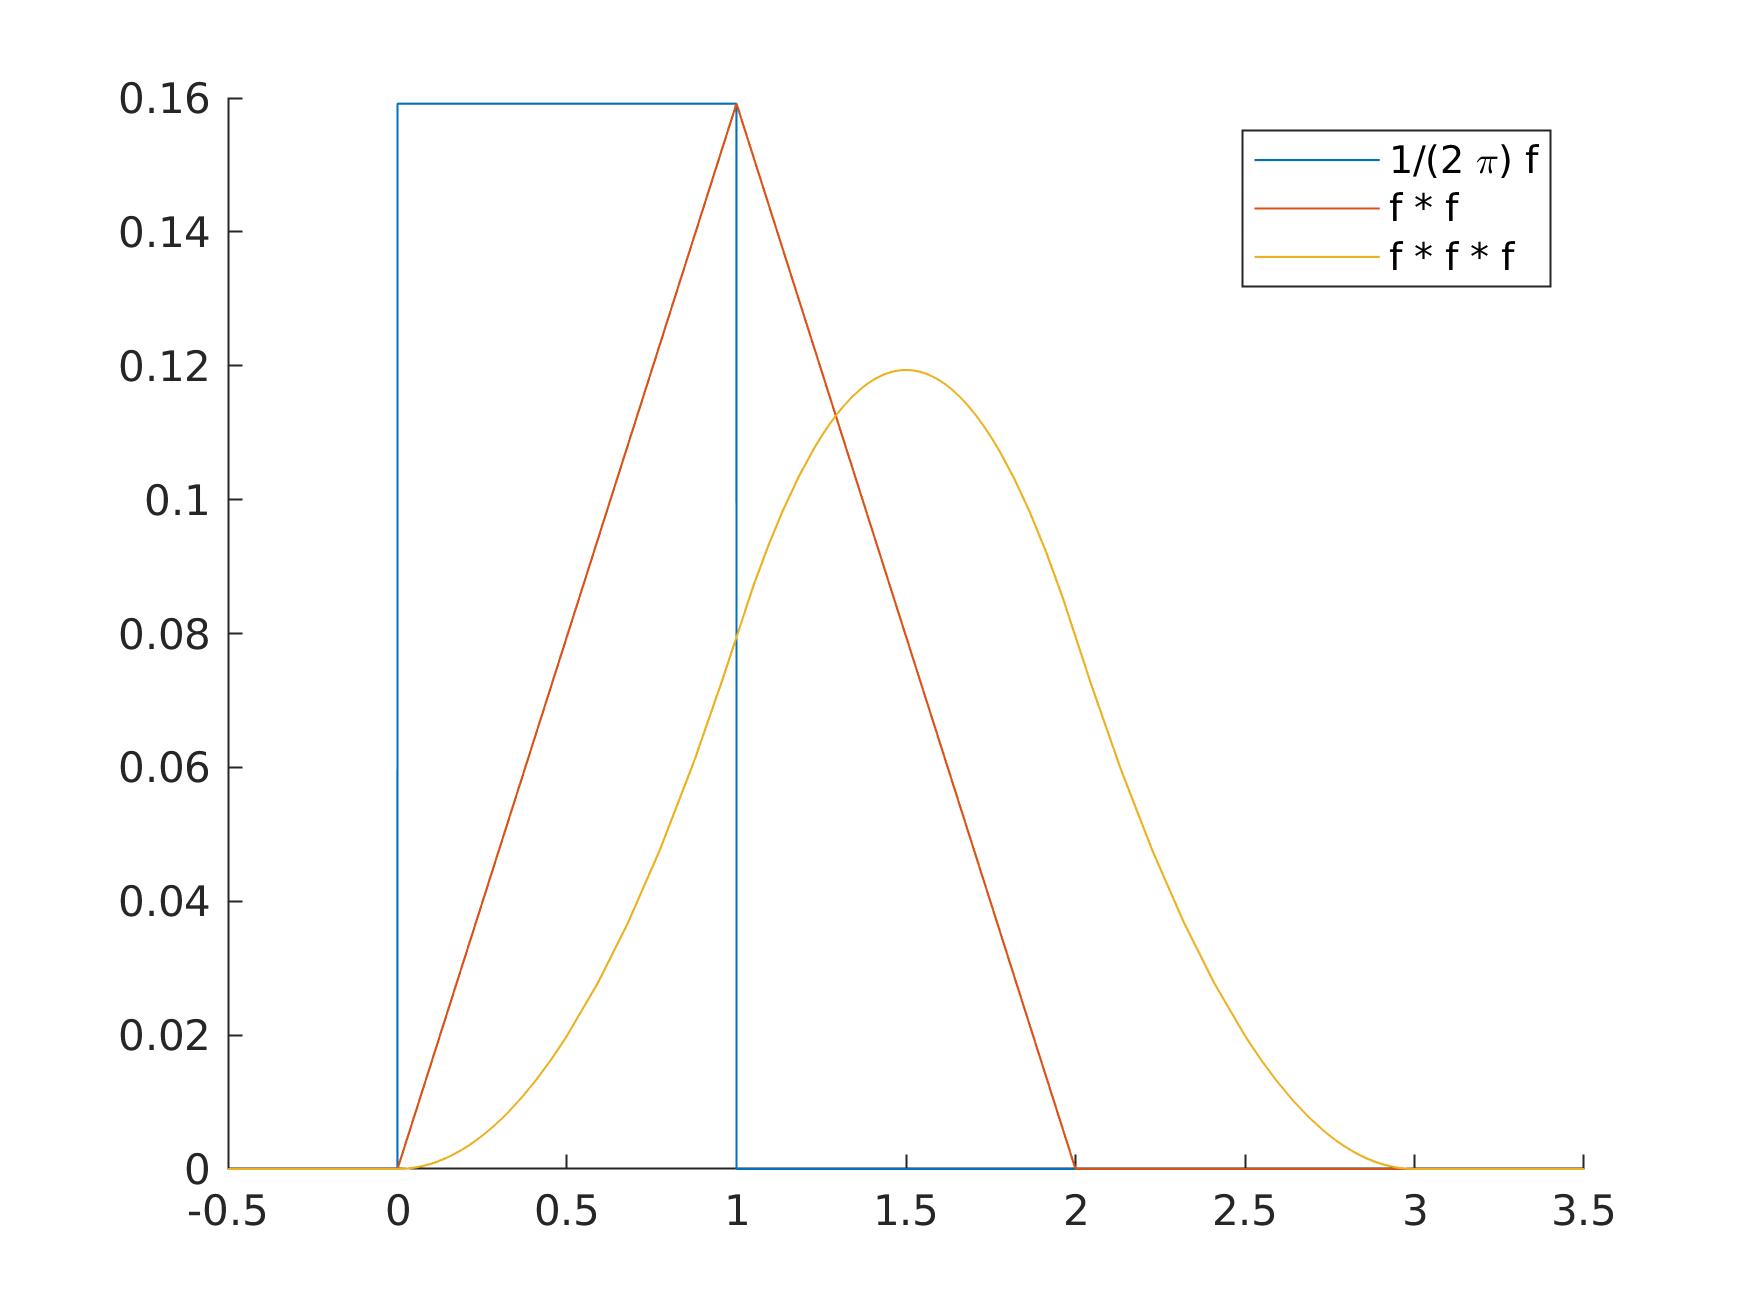
\includegraphics[width=5in]{q48}
    \centering
    \caption{Convolutions of $f$}
    \label{fig:4-8}
\end{figure}

\newpage

\lstinputlisting[caption={Code to generate plot},captionpos=b,label={lst:1}]{./code/q48.m}

\newpage

4.17. Show that if $f$ is integrable and $P \in \Pc_N$, then $f * P \in \Pc_N$.

\textit{Solution.}
If $P \in \Pc_N(\T)$ then we can express
%
\begin{equation*}
    \sum_{|n| \leq N} a_n e^{i n \theta}
\end{equation*}
%
for some set of coefficients $\cbr{a_n}_{n \in \N} \subset \C$. Because
$f$ is integrable we have that
%
\begin{equation*}
    \envert{\int_{-\pi}^\pi f(y) e^{-i n y} \dif y}
    \leq \int_{-\pi}^\pi |f(y)| |e^{-i n y}| \dif y
    = \int_{-\pi}^\pi |f(y)| \dif y
    < \infty
    .
\end{equation*}
%
Define
%
\begin{equation*}
    c_n \coloneqq \frac{1}{2 \pi} a_n \int_{-\pi}^\pi f(y) e^{-i n y} \dif y
    ,
\end{equation*}
%
each of which is finite as shown by our calculation above. Then we have that
%
\begin{align*}
    (f * P) (\theta)
        &= \frac{1}{2 \pi} \int_{-\pi}^\pi f(y) P(\theta - y) \dif y \\
        &= \frac{1}{2 \pi} \int_{-\pi}^\pi f(y) \del{\sum_{|n| \leq N} a_n e^{i n (\theta - y)}} \dif y \\
        &= \frac{1}{2 \pi} \sum_{|n| \leq N} \del{a_n  \int_{-\pi}^\pi f(y) e^{-i n y} \dif y} e^{i n \theta} \\
        &= \sum_{|n| \leq N} c_n e^{i n \theta}
        .
\end{align*}
%
Clearly we have that $f * P \in \Pc_N$.

\newpage

4.22. Suppose $K$ is a continuous function on $\R$ that is zero for all
$|\theta| \geq \pi$. Assume $\int_{- \pi}^\pi K(\theta) \dif \theta = 2 \pi$.
Let $K_n \coloneqq n K(n \theta)$ for $- \pi \leq \theta \leq \pi$. Verify
that $\cbr{K_n}_{n \geq 1}$ is a family of good kernels on $\T$.

\textit{Solution.}
For $\cbr{K_n}_{n \geq 1}$ to be a family of good kernels on $\T$ we require

\begin{adjustwidth}{2.5em}{0pt}
    (a) For all $n \in \N$, $\frac{1}{2 \pi} \int_{- \pi}^\pi K_n(\theta) \dif \theta = 1$;

    (b) There exists $M > 0$ so that
    $\int_{- \pi}^\pi |K_n(\theta)| \dif \theta \leq M$ for all $n \in \N$;

    (c) For each $\delta > 0$,
    $\int_{\delta \leq |\theta| \leq \pi} |K_n(\theta)| \dif \theta \to 0$ as $n \to \infty$.
\end{adjustwidth}

For property (a) we have that
%
\begin{align*}
    \frac{1}{2 \pi} \int_{- \pi}^\pi K_n(\theta) \dif \theta
        &= \frac{1}{2 \pi} \int_{- \pi}^\pi n K(n \theta) \dif \theta \\
        &= \frac{1}{2 \pi} \int_{- n \pi}^{n \pi} K(x) \dif x \\
        &= \frac{1}{2 \pi} \int_{-\pi}^{\pi} K(x) \dif x \\
        &= \frac{1}{2 \pi} \cdot 2 \pi = 1
        ,
\end{align*}
%
where in the second line we used the substitution $x = n \theta$ and in
the third line we used that $K(\theta) = 0$ for $|\theta| \geq \pi$.

For property (b) we use that $K$ is integrable on $[-\pi, \pi]$ (because
it is continuous and the interval is closed) and hence there exists a
constant $M > 0$ such that
%
\begin{equation*}
    \int_{- \pi}^\pi |K(\theta)| \dif \theta < M
    .
\end{equation*}
%
Then we have for all $n \in \N$ that, using the same tricks we used
in proving property (a),
%
\begin{align*}
    \int_{- \pi}^\pi |K_n(\theta)| \dif \theta
        &= \int_{- \pi}^\pi |n K(n \theta)| \dif \theta \\
        &= \int_{- \pi}^\pi n |K(n \theta)| \dif \theta \\
        &= \int_{- n \pi}^{n \pi} |K(x)| \dif x \\
        &= \int_{-\pi}^{\pi} |K(x)| \dif x < M
        ,
\end{align*}
%
which proves property (b).

For property (c), fix any $\delta > 0$ with $\delta \leq \pi$. Then we
have that
%
\begin{align*}
    \int_{\delta \leq |\theta| \leq \pi} |K_n(\theta)| \dif \theta
        &=
        \int_{- \pi}^{-\delta} |K_n(\theta)| \dif \theta
        +
        \int_{\delta}^{\pi} |K_n(\theta)| \dif \theta
        \\
        &=
        \int_{- \pi}^{-\delta} |n K(n \theta)| \dif \theta
        +
        \int_{\delta}^{\pi} |n K(n \theta)| \dif \theta
        \\
        &=
        \int_{- \pi}^{-\delta} n |K(n \theta)| \dif \theta
        +
        \int_{\delta}^{\pi} n |K(n \theta)| \dif \theta
        \\
        &=
        \int_{- n \pi}^{-n \delta} |K(x)| \dif x
        +
        \int_{n \delta}^{n \pi} |K(x)| \dif x
    .
\end{align*}
%
By taking $n$ sufficiently large, we can guarantee that
%
\begin{equation*}
    \del{[- n \pi, - n \delta] \cup [n \delta, n \pi]} \cap [- \pi, \pi] = \emptyset
    .
\end{equation*}
%
and hence $K$ is zero within our limits of integration above if we take
$n$ large enough (recall that $K$ is zero outside of $[- \pi, \pi]$). Therefore
%
\begin{equation*}
    \int_{\delta \leq |\theta| \leq \pi} |K_n(\theta)| \dif \theta
        =
        \int_{- n \pi}^{-n \delta} |K(x)| \dif x
        +
        \int_{n \delta}^{n \pi} |K(x)| \dif x
        = 0 + 0 = 0
\end{equation*}
%
as $n \to \infty$. This proves property (c).

\newpage

4.31. Show that the Fejér kernel $F_N$ is a good kernel and that
$\sigma_N f = F_N * f$.

\textit{Solution.}
To show that $F_N$ is a good kernel we need to prove the three
properties listed in the solution to the previous question (4.22).
The kernel $F_N$ is given by
%
\begin{equation*}
    F_N(\theta) \coloneqq \frac{1}{N} \sum_{n = 0}^{N - 1} D_n (\theta)
    ,
\end{equation*}
%
where $D_n$ is the $n$th Dirichlet kernel. In part (c) we'll use the
following expression of $F_N$ from the course textbook:
%
\begin{equation}
    F_N(\theta) = \frac{1}{N} \sbr{\frac{\sin \del{\frac{N \theta}{2}}}{\sin \del{\frac{\theta}{2}}}}^2
    \label{eq:431z}
    .
\end{equation}
%
For property (a) we'll use Theorem 4.3 from the course textbook, which tells us
that
%
\begin{equation*}
    \int_{- \pi}^\pi D_N(\theta) \dif \theta = 2 \pi
\end{equation*}
%
for all $N \geq 0$. Thus
%
\begin{align*}
    \frac{1}{2 \pi} \int_{- \pi}^\pi F_N(\theta) \dif \theta
        &= \frac{1}{2 \pi} \int_{- \pi}^\pi
            \frac{1}{N} \sum_{n = 0}^{N - 1} D_n(\theta)
            \dif \theta \\
        &= \frac{1}{2 \pi} \frac{1}{N} \sum_{n = 0}^{N - 1}
            \int_{- \pi}^\pi D_n(\theta) \dif \theta \\
        &= \frac{1}{2 \pi} \frac{1}{N} \sum_{n = 0}^{N - 1} 2 \pi \\
        &= \frac{1}{2 \pi} \frac{1}{N} N 2 \pi \\
        &= 1
        ,
\end{align*}
%
which proves property (a).

Noting that $|F_N(\theta)| = F_N(\theta)$ (this can be seen clearly
from~\eqref{eq:431z}), property (b) follows directly from property (a).

For property (c), fix $\delta > 0$ where $\delta \leq \pi$. For
this proof we'll use two facts. The first fact is that for all
$x \in \R$
%
\begin{equation}
    \sin^2(x) \leq 1
    \label{eq:431a}
\end{equation}
%
The second fact is that for all $\theta \in [\delta, \pi]$,
%
\begin{equation}
    \frac{1}{\sin^2 \del{\frac{\theta}{2}}}
    \leq \frac{1}{\sin^2 \del{\frac{\delta}{2}}}
    \label{eq:431b}
    .
\end{equation}
%
This is because for all $\theta_1, \theta_2 \in [0, \pi/2]$,
if $\theta_1 \leq \theta_2$ then $\sin(\theta_1) \leq \sin(\theta_2)$.
In our fact above we have that
$\frac{\theta}{2}, \frac{\delta}{2} \in [0, \pi / 2]$,
and $\frac{\delta}{2} \leq \frac{\theta}{2}$, so
$\sin (\frac{\delta}{2}) \leq \sin (\frac{\theta}{2})$. After taking
reciprocals and squaring, we obtain~\eqref{eq:431b}.

Now to prove property (c), we have
%
\begin{align*}
    \int_{\delta \leq |\theta| \leq \pi} |F_N(\theta)| \dif \theta
        &= \int_{\delta \leq |\theta| \leq \pi} F_N(\theta) \dif \theta \\
        &= \int_{\delta \leq |\theta| \leq \pi}
            \frac{1}{N} \sbr{\frac{\sin \del{\frac{N \theta}{2}}}{\sin \del{\frac{\theta}{2}}}}^2
            \dif \theta \\
        &= \frac{1}{N} \int_{\delta \leq |\theta| \leq \pi}
            \sbr{\frac{\sin \del{\frac{N \theta}{2}}}{\sin \del{\frac{\theta}{2}}}}^2
            \dif \theta \\
        &\leq \frac{1}{N} \int_{\delta \leq |\theta| \leq \pi}
            \frac{1}{\sin^2 \del{\frac{\theta}{2}}}
            \dif \theta \\
        &\leq \frac{1}{N} \int_{\delta \leq |\theta| \leq \pi}
            \frac{1}{\sin^2 \del{\frac{\delta}{2}}}
            \dif \theta \\
        &= \frac{2 (\pi - \delta)}{N \sin^2 \del{\frac{\delta}{2}}}
        \to 0 \text{ as } N \to \infty
    ,
\end{align*}
%
where in the fourth line we used~\eqref{eq:431a} and in the fifth line
we used~\eqref{eq:431b}.

Finally, to show $\sigma_N f = F_N * f$, we have that
%
\begin{align*}
    (F_N * f) (\theta)
        &= \frac{1}{2 \pi} \int_{- \pi}^\pi f(y) F_N(\theta - y) \dif y \\
        &= \frac{1}{2 \pi} \int_{- \pi}^\pi f(y) \del{\frac{1}{N} \sum_{n = 0}^{N - 1} D_n (\theta - y)} \dif y \\
        &= \frac{1}{N} \sum_{n = 0}^{N - 1} \frac{1}{2 \pi} \int_{- \pi}^\pi f(y) D_n (\theta - y) \dif y \\
        &= \frac{1}{N} \sum_{n = 0}^{n - 1} \frac{1}{2 \pi} \int_{- \pi}^\pi f(y) \del{\sum_{|k| \leq n} e^{i k (\theta - y)}} \dif y \\
        &= \frac{1}{N} \sum_{n = 0}^{n - 1} \sum_{|k| \leq n} e^{i k \theta} \frac{1}{2 \pi} \int_{- \pi}^\pi f(y) e^{- i k y} \dif y \\
        &= \frac{1}{N} \sum_{n = 0}^{n - 1} \sum_{|k| \leq n} e^{i k \theta} \widehat{f}(k)  \\
        &= \frac{1}{N} \sum_{n = 0}^{n - 1} S_n f(\theta) \\
        &\eqqcolon \sigma_N f
        .
\end{align*}


\newpage

5.16. Fix $g \in L^2(\T)$. Suppose that $f, h_k \in L^2(\T)$ for $k \in \Z$,
and that $f = \sum_{k = 1}^\infty h_k$ in the $L^2$ sense. Show that
$\sum_{k = 1}^\infty \langle g, h_k \rangle = \langle g, \sum_{k = 1}^\infty h_k \rangle$.

\textit{Solution.}
Let $f_n = \sum_{k = 1}^n h_k$. Since each $h_k \in L^2(\T)$, we
have that each $f_n \in L^2(\T)$; also, we have that $f_n \to f$ as
$n \to \infty$. Therefore, using Proposition 5.15 from the course textbook,
we have
%
\begin{align*}
    \sum_{k = 1}^\infty \langle g, h_k \rangle
        &= \lim_{n \to \infty} \sum_{k = 1}^n \langle g, h_k \rangle \\
        &= \lim_{n \to \infty} \langle g, \sum_{k = 1}^n h_k \rangle \\
        &= \lim_{n \to \infty} \langle g, f_n \rangle \\
        &= \langle g, \lim_{n \to \infty} f_n \rangle \\
        &= \langle g, f \rangle \\
        &= \langle g, \sum_{k = 1}^\infty h_k \rangle
        .
\end{align*}

\newpage

5.17. Let $\cbr{e_n}_{n \in \Z}$ be the set of trigonometric functions.
Suppose that $\cbr{a_n}_{n \in \Z}$, $\cbr{b_n}_{n \in \Z}$ are sequences
of complex numbers, $f = \sum_{n \in \Z} a_n e_n$, and
$g = \sum_{n \in \Z} b_n e_n$, where the equalities are in the $L^2$ sense.
Show that $\langle f, g \rangle = \sum_{n \in \Z} a_n \overline{b}_n$.
In particular, show that $\norm{f}^2_{L^2(\T)} = \sum_{n \in \Z} |a_n|^2$.

\textit{Solution.}
This is easy to show by remembering that
%
\begin{equation*}
    \frac{1}{2 \pi} \int_{-\pi}^{\pi} e^{i (n - k) \theta} \dif \theta = \delta_{n, k}
    .
\end{equation*}
%
Let $f_n = \sum_{|k| < n} a_k e_k$, and $g_n = \sum_{|k| < n} b_k e_k$. Then,
again using Proposition 5.15 from the course textbook we have
%
\begin{align*}
    \langle f, g \rangle
        &= \lim_{N \to \infty} \lim_{K \to \infty} \langle f_N, g_K \rangle \\
        &= \lim_{N \to \infty} \lim_{K \to \infty} \frac{1}{2 \pi} \int_{- \pi}^\pi f_N(\theta) \overline{g_K(\theta)} \dif \theta \\
        &= \lim_{N \to \infty} \lim_{K \to \infty} \frac{1}{2 \pi} \int_{- \pi}^\pi \del{\sum_{|n| \leq N} a_n e^{i n \theta}} \overline{\del{\sum_{|k| \leq K} b_k e^{i k \theta}}} \dif \theta \\
        &= \lim_{N \to \infty} \lim_{K \to \infty} \frac{1}{2 \pi} \int_{- \pi}^\pi \del{\sum_{|n| \leq N} a_n e^{i n \theta}} \del{\sum_{|k| \leq K} \overline{b_{k}} e^{-i k \theta}} \dif \theta \\
        &= \lim_{N \to \infty} \lim_{K \to \infty} \frac{1}{2 \pi} \int_{- \pi}^\pi \sum_{|n| \leq N} \sum_{k \leq K} a_n \overline{b_{k}} e^{i (n - k) \theta} \dif \theta \\
        &= \lim_{N \to \infty} \lim_{K \to \infty} \sum_{|n| \leq N} \sum_{|k| \leq K} a_n \overline{b_{k}} \del{\frac{1}{2 \pi} \int_{- \pi}^\pi e^{i (n - k) \theta} \dif \theta} \\
        &= \sum_{n \in \Z} \sum_{k \in \Z} a_n \overline{b_{k}} \del{\frac{1}{2 \pi} \int_{- \pi}^\pi e^{i (n - k) \theta} \dif \theta} \\
        &= \sum_{n \in \Z} \sum_{k \in \Z} a_n \overline{b_{k}} \delta_{n, k} \\
        &= \sum_{n \in \Z} a_n \overline{b_{n}}
        .
\end{align*}

To show that $\norm{f}^2_{L^2(\T)} = \sum_{n \in \Z} |a_n|^2$, recall
that for any $c \in \C$, $c \overline{c} = |c|^2$. Hence we have
%
\begin{align*}
    \norm{f}^2_{L^2(\T)}
        &= \del{\langle f, f \rangle^{1/2}}^2 \\
        &= \langle f, f \rangle \\
        &= \sum_{n \in \Z} a_n \overline{a_{n}} \\
        &= \sum_{n \in \Z} |a_n|^2
        .
\end{align*}

\end{document}
